\iffalse
\documentclass[12pt]{article}
\usepackage{graphicx}
\usepackage{amsmath}
\usepackage{mathtools}
\usepackage{gensymb}

\newcommand{\mydet}[1]{\ensuremath{\begin{vmatrix}#1\end{vmatrix}}}
\providecommand{\brak}[1]{\ensuremath{\left(#1\right)}}
\providecommand{\norm}[1]{\left\lVert#1\right\rVert}
\newcommand{\solution}{\noindent \textbf{Solution: }}
\newcommand{\myvec}[1]{\ensuremath{\begin{pmatrix}#1\end{pmatrix}}}
\let\vec\mathbf

\begin{document}
\begin{center}
\textbf\large{CHAPTER-7 \\ COORDINATE GEOMETRY}
\end{center}
\section*{Excercise 7.2}

Q3. Find the area of the triangle formed by joining the mid-points of the sides of the triangle
whose vertices are $\vec(0, –1), \vec(2, 1) \text{ and } \vec(0, 3)$. Find the ratio of this area to the area of the
given triangle
\\
\solution
\\
\fi
The coordinates are given as
	\begin{align}
	\vec{A} = \myvec{
		0\\
		-1\\
		},
	\vec{B} = \myvec{
		2\\
		1\\
		},
	\vec{C} = \myvec{
		0\\
		3\\
		}
	\end{align}
Calculating midpoints,
	\begin{align}
		\vec{P} = \frac{1}{2}\vec(\vec{A}+\vec{B}) = \frac{1}{2}\myvec{2\\0\\} = \myvec{1\\0\\}\\
		\vec{Q} = \frac{1}{2}\vec(\vec{B}+\vec{C}) = \frac{1}{2}\myvec{2\\4\\} = \myvec{1\\2\\}\\
		\vec{R} = \frac{1}{2}\vec(\vec{A}+\vec{C}) = \frac{1}{2}\myvec{0\\2\\} = \myvec{0\\1\\}
	\end{align}
	Since
	\begin{align}
		\vec{P}-\vec{Q} &=  \myvec{
  1 \\
  0 
 } - \myvec{
  1 \\
  2 
 } = \myvec{
 0 \\
 -2 
 }
		\\
		\vec{Q}-\vec{R} &=  \myvec{
  1 \\
  2 \\
 } - \myvec{
  0 \\
  1 \\
 } = \myvec{
 1 \\
 1 \\
 }
	\end{align}
	the area is obtained as
	\begin{align}
		ar(PQR)&=\frac{1}{2}{\norm{\vec(\vec{P}-\vec{Q})\times\vec(\vec{Q}-\vec{R})}}
		\\
		&=\frac{1}{2}\mydet{0 & 1\\-2 & 1}
		=1
	\end{align}
	Similarly, 
	\begin{align}
		\vec{A}-\vec{B} &=  \myvec{
  0 \\
  -1 \\
 } - \myvec{
  2 \\
  1 \\
 } = \myvec{
 -2 \\
 -2 \\
 }
 \\
		\vec{A}-\vec{C} &=  \myvec{
  0 \\
  -1 \\
 } - \myvec{
  0 \\
  3 \\
 } = \myvec{
 0 \\
 -4 \\
 }
	\end{align}
 the area is obained as
	\begin{align}
		ar(ABC)&=\frac{1}{2}{\norm{\vec(\vec{A}-\vec{B})\times\vec(\vec{A}-\vec{C})}}\\
		&=\frac{1}{2}\mydet{-2 & 0\\-2 & -4}
=4
	\end{align}
	Thus, the resultant ratio of two areas is 1:4.
	See Fig.
\ref{fig:10/7/3/3Fig}
\begin{figure}[!h]
	\begin{center} 
	    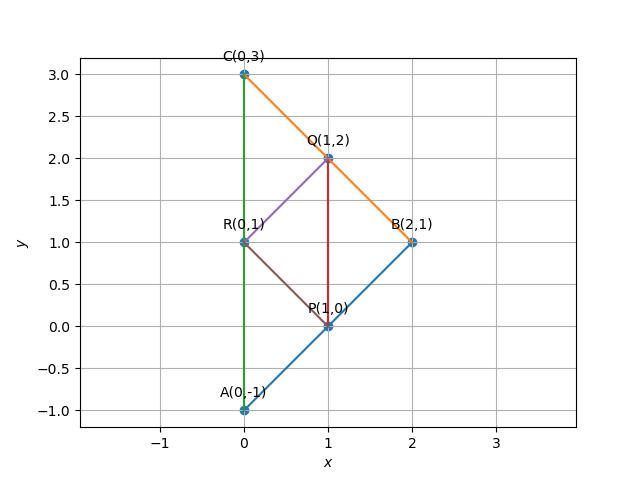
\includegraphics[width=\columnwidth]{chapters/10/7/3/3/figs/trigraph.png}
	\end{center}
\caption{}
\label{fig:10/7/3/3Fig}
\end{figure}
